\chapter{Materiais}
\begin{itemize} %% TODO: colocar as rodas: http://www.hobbyking.com/hobbyking/store/__2176__598__Hardware_Accessories-Wheels_0_40mm.html
 \item 5 sensores ultrassônicos de distância HC-SR04
 \item 2 motores \textit{brushless outrunner} Turnigy D2836/9 950KV
 \item 2 \textit{Electronic Speed Controlers (ESCs) Hobby King} com UBEC de 5.5V/4A: um de 35A e outro de 40A 
 \item 2 módulos de rádio frequência baseados no \textit{transceiver} Nordic nRF24L01+ 
 \item bateria LiPo 30C de 2800 mAh
 \item 1 Arduino Uno
 \item 1 Arduino Pro Mini
 \item 1 Conversor/Adaptador USB-Serial PL2303
 \item 1 Carregador IMAX B6-AC
\end{itemize}

\section{Motor \textit{Brushless}}
São motores síncronos\footnote{Motores Síncronos: o campo magnético girante do rotor e do estator têm a mesma frequência.} de corrente contínua cuja 
comutação é feita eletronicamente e não mecanicamente por meio de escovas como nos motores CC comuns, por isso denominados \textit{brushless}.
Possui aplicações nas indústrias de automóveis, aeroespacial, médica, de equipamentos de automação industrial e instrumentação .
Os motores BLDC apresentam algumas vantagens em relação aos de corrente contínua comutados e de indução no que concerne a: resposta dinâmica, ruídos 
de operação, durabilidade (i.e. vida útil), assim como razão do torque pelas dimensões do motor \cite{motor_2}. 

O seu rotor consiste de um imã permanente, enquanto seu estator apresenta pólos formados por enrolamentos. Como é preciso que os enrolamentos sejam 
energizados na sequência correta para que um campo magnético girante seja criado de modo a produzir o maior torque. Nas máquinas CC isto é feito 
mecanicamente através das escovas, mas no caso do BLDC é preciso que a posição do rotor em relação ao estator seja conhecida para que então se faça o 
acionamento na ordem correta. Existem dois meios de se obter esta informação: sensores de efeito hall, método empregado neste trabalho, ou 
processamento da força contra eletromotriz dos enrolamentos do estator.

Sensores de efeito Hall são transdutores analógicos que relacionam a intensidade do campo magnético externo transversalmente disposto a ele em termos 
de tensão elétrica. Quando associado a um circuito comparador \textit{schmitt trigger}, comporta-se como um sensor digital que aponta quando a 
intensidade do campo magnético atinge um valor de limiar pré-determinado. Ao dispor sensores deste tipo ao longo do estator, torna-se possível uma 
estimativa da posição do rotor ao ser feito um estudo comparativo da resposta de cada sensor, cruzando esta informação com a posição que 
cada um destes se encontra em relação ao estator \cite{motor_1}.

Há a possibilidade de fazer a comutação sem empregar qualquer tipo de sensor, logo, trata-se de um método mais barato. 
Nesse caso, a estimativa da posição do rotor se dá através do processamento das forças contra-eletromotriz de cada um dos enrolamentos do estator.
No entanto, algumas limitações surgem: o motor deve operar acima de uma dada rotação, caso contrário o método não funciona; mudanças bruscas de carga 
não podem ocorrer; há discontinuidades na resposta do motor quando operando em velocidades acima da taxa de comutação ideal \cite{motor_1}.

\section{ESC}
Controlador responsável por processar as informações oriundas dos sensores de efeito Hall do motor BLDC e providenciar o acionamento correto 
dos enrolamentos do estator para que a velocidade angular se dê de acordo com o sinal de controle é enviado a este dispositivo.
No caso dos ESCs utilizados no presente trabalho, este sinal de controle é feito utilizando-se modulação por largura de pulso, i.e. PWM. 
A frequência de operação varia de acordo com o modelo do controlador e para o caso deste projeto é de 400Hz.
%% TODO: \cite{carlson}
%% TODO: fazer uma descrição mais rica de como funciona este dispositivo.
%% TODO: citar que toda a programação do ESC é feita via pwm.
\section{Sensor Ultrassônico}

\subsection{Princípio de Funcionamento}
Utiliza o método \textit{time of flight}, que consiste na medição do intervalo de tempo, igualmente denominado \textit{time of flight}, que uma onda 
ou partícula leva para percorrer uma determinada distância em um dado meio. 
Pode ser utilizado para medir: distância, velocidade \cite{TOF_velocity}, propriedades do meio de propagação ou da partícula propagante
\cite{TOF_medium1,TOF_medium2}.

Para medidores de proximidade, como é o caso de sonares e lasers, um transdutor emissor faz a conversão do sinal elétrico, denominado 
\textit{trigger}, em um pulso de ondas (acústicas para o caso do sonar e eletromagnéticas para o laser), dando início à medição de tempo.
Quando esta onda propagante encontra um objeto que a reflita de volta ao sensor e a intensidade deste sinal recebido, denominado \textit{echo}, está 
acima de um determinado valor de limiar, o transdutor receptor envia um sinal elétrico que interrompe a contagem de tempo, obtendo-se 
assim a medida do \textit{time of flight}, $\tau$.
Com isso, supondo que a velocidade de propagação, $\nu$, da onda em questão no meio seja conhecida, de acordo com \cite{siegwart}, pode-se 
calcular a distância, $\Delta$, entre o sensor e o objeto que reflete o pulso de ondas pela equação \ref{TOF_eq}:
\begin{equation}
 \label{TOF_eq}
 \Delta = \frac{\nu \times \tau }{2}
\end{equation}

Quanto ao sensor ultrassonico especificamente, temos que as ondas sonoras utilizadas estão usualmente situadas entre 40kHz e 180kHz, sendo 
emitidas no formato de pacotes compostos por uma série de pulsos; no caso do sonar utilizado neste trabalho, 8 pulsos de 40kHz. 
Por se tratarem de ondas mecânicas, é importante que a tensão de limiar, do inglês \textit{threshold}, decresça ao longo do ciclo de 
leitura da seguinte forma \cite{siegwart}: 
durante o período denominado \textit{blanking time}\cite{siegwart}  ou \textit{dead time}\cite{murphy} na literatura, o qual engloba o intervalo de 
emissão das ondas sonoras até o momento em que o 
diafragma para de oscilar (o que pode constituir alguns milisegundos após a cessação do sinal de \textit{trigger}), a tensão de limiar é muito alta 
no intuito de eliminar leituras inválidas decorrentes de interferência entre emissor e receptor; em seguida, a tensão de \textit{threshold} se reduz 
a um valor que permita detecção de obstáculos e vai sendo continuamente decrementada com o passar do tempo. 
Isso se dá pelo fato de que a intensidade do sinal acústico, i.e. potência por ângulo sólido, sofre atenuações atmosférica que variam com a 
distância percorrida, conforme a equação \ref{Atm_Attenuation} \cite{everett}, que leva em consideração somente efeitos da divergência esférica e 
absorção molecular.
\begin{equation}
 \label{Atm_Attenuation}
 I = \frac{ I_0 e^{-2 \alpha R} }{4 \pi R^2}
\end{equation}
Em que: $\alpha$ é o coeficiente de atenuação do meio, associado às absorções moleculares, o qual varia em função da frequência da onda emitida 
assim como de propriedades do meio, e.g. humidade e poeira contida no ar.
Para ondas de 40kHz: $0,197\frac{dB}{m} < \alpha < 0,295 \frac{dB}{m}$. % TODO posso deixar essa desigualdade aqui???

\subsection{Limitações}

\subsubsection{Variação na velocidade de propagação da onda acústica}
Como citado anteriormente, a medição da distância pressupõe que a velocidade de propagação da onda no meio é conhecida. 
No entanto, mudanças na temperatura e umidade do fluido em que a onda se propaga podem causar erros de medida não desprezíveis \cite{everett}.

\subsubsection{Direcionalidade}
O emissor da radiação acústica ultrassônica apresenta um padrão de radiação\cite{balanis,pozar} composto por lobos laterais\cite{balanis,pozar} que 
não são levados em conta, pois a maioria dos sistemas supõem toda radiação recebida como oriunda do lobo central\cite{balanis,pozar}, usualmente 
modelado como um cone de aproximadamente $30^o$ que varre até 5 metros \cite{murphy}. De acordo com \cite{HC-SR04}, para o dispositivo utilizado 
nesse trabalho o ângulo de abertura do feixe é de $15^o$ e o alcance, 4 metros.

Além deste problema, o próprio fato de que direcionalidade do sensor é baixa, i.e. o lobo central é largo, implica numa 
imprecisão na medida obtida, pois não é possível associar a distância lida a um lugar específico, mas sim à região no espaço coberta pelo lobo 
central \cite{siegwart}.

\subsubsection{Resposta no Ambiente Alvo}
Por ser um sensor refletivo, a performance do sonar é significativamente afetada pelas características do alvo \cite{everett}.
Um dos problemas decorrentes desse fato é que determinados objetos apresentam elevada taxa de absorção ou, ao contrário, são atravessados pela 
radiação o que resulta, em ambos os casos, que pouca ou nenhuma energia retorna ao sensor. Dessa forma, estes objetos são invisíveis para o dado 
método de medição; materiais como espuma, pele e roupas podem absorver as ondas acústicas \cite{siegwart} enquanto objetos com áreas superficiais 
pequenas, e.g. mesas e cadeiras, podem não ser detectados \cite{murphy}. Vale ressaltar que as propriedades de relexão, absorção e transmissão 
são variáveis com a frequência e do tipo de radiação, acústica ou eletromagnética.
%% TODO achar alguém que falou isso e explica absorção reflexão e transmissão
Existem outros problemas relativos ao ambiente alvo que não são relacionados à absorção ou transmissão da radiação, mas à reflexão serão tratados nas 
seções subsequentes separadamente.

\subsubsection{\textit{Foreshortening}}
Como a direticionalidade dos sensores ultrassônicos é baixa, isto é a largura de feixe do lobo central é alta, aproximadamente $30^o$, quando o alvo 
a ser detectado não está perpendicularmente posicionado em relação ao eixo acústico do sensor, o cone que formado pelo lobo principal atinge o objeto 
em instantes diferentes. Consequentemente, retorna ao sensor em instantes diferentes provocando um desvio na leitura da distância, fazendo com que o 
obstáculo pareça estar mais próximo do que está na realidade. Por isso este problema é denominado \textit{foreshortening}

\subsubsection{Reflexão especular}
Dentro desta mesma situação em que o obstáculo não está perpendicular ao eixo acústico do sonar, existe a possibilidade de que a onda emitida seja 
refletida de tal forma que não retorne ao sensor, caso este em que o obstáculo não é percebido. Outra hipótese é de que esta onda refletida 
para longe do sensor atinja outra(s) superfície(s) até que retorne ao sensor, desta forma a medida obtida indica que o alvo encontra-se mais distante 
do que realmente está \cite{roseli,siegwart,everett}.  

\subsubsection{\textit{Crosstalk}}
Quando utiliza-se uma matriz de sensores ultrassônicos, o problema da relexão especular é agravado, pois pode constituir interferência entre 
sensores. De modo que além da medida feita estar errada, o posicionamento do obstáculo será também errôneo \cite{murphy}. No entanto, diferentemente 
da reflexão especular, este problema pode ser amenizado de diferentes maneiras, vide \cite{2016_artigo_1,2016_artigo_5}

\subsubsection{Tempo de Resposta} %% TODO:


\section{Módulo de rádio frequência}

  \begin{figure}[!htb] %% TODO ver a fonte dessa figura
    \centering
    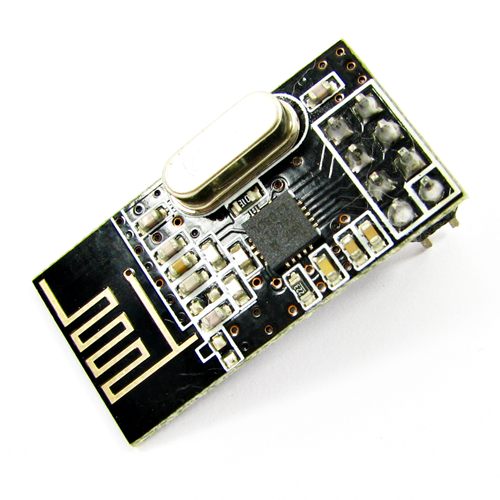
\includegraphics[width=0.7\linewidth]{../../Imagens/nordicc.png}
    \caption{Módulo de Rádio Frequência baseado no \textit{transceiver} da Nordic nRF24L01+}
    \label{Nordic}
  \end{figure}
Módulo de rádio frequência ( Fig. \ref{Nordic}) de baixo custo e consumo cuja faixa de operação situa-se na banda S das ondas UHF ( \textit{Ultra 
High Frequency} ), com uma porção dentro da banda ISM \footnote{maiores informações no apêndice}.
Algumas informações técnicas \cite{nRF} de interesse estão listadas abaixo: 
\begin{itemize}
 \item Tensão de alimentação: 1,9V - 3,6V
 \item Antena em circuito impresso do tipo MIFA(\textit{Meandered Inverted-F Antenna}) \cite{MIFA}
 \item Frequência de operação: 2,4GHz - 2,525GHz
 \item Modulação digital do tipo GFSK \footnote{maiores informações no apêndice}
 \item Apresenta até 126 canais de comunicação \footnote{Válido apenas para as taxas de 250kbps e 1 Mbps; a 2Mbps este valor cai à metade, i.e. 63 
canais.}
 \item Taxas de bits: 250kbps, 1Mbps ou 2Mbps
 \item Potências de saída de transmissão: 0dBm, -6dBm, -12dBm e -18dBm
 \item Interface com o microcontrolador por SPI \footnote{maiores informações no apêndice} à taxa de até 10Mbps
 \item Pinos de entrada tolerantes a até 5V
 \item 
Pacotes recebidos verificados automaticamente , certificando-se da validade do endereço apontado e legitimando a integridade 
do pacote via CRC(\textit{Cyclic Redundancy Check}) \footnote{Vide apêndice para uma breve explanação sobre CRC}, antes de 
serem movidos às filas de dados recebidos (\textit{RX FIFO})
 \item Receptor envia ao transmissor um pacote de confirmação de recepção dos dados pelo mesmo canal (\textit{acknowledgment packet}).
\end{itemize}

\section{Arduino}
\subsection{Arduino Uno}
Trata-se de uma plataforma de prototipação eletrônica aberta, i.e. \textit{open-source hardware}, baseada no microcontrolador de 8 bits da Atmel 
ATMega328P \cite{ATMega}, programável via USB ou serial (ICSP) através de um microcomputador, por exemplo, por meio do ambiente de desenvolvimento 
\textit{Arduino Software IDE}, \textit{open-source software} e encontra-se no GitHub \cite{ArduSoft}.
Algumas informações técnicas \cite{ArduInfo} de interesse estão listadas abaixo: 
\begin{itemize}
 \item Dimensões: 53.4mm x 68.6mm
 \item Tensão de alimentação recomendável: 7V - 12V
 \item Fonte de tensão de 3,3V embutida
 \item Memória 
 \begin{itemize}
  \item Flash: 32kB 
  \item SRAM: 2kB
  \item EEPROM: 1kB
 \end{itemize}

 \item 20 portas digitais de entrada/saída, das quais 6 podem ser usadas como saídas PWM
 \item 6 portas de entrada analógicas
 \item \textit{clock} de 16MHz
\end{itemize}

\subsection{Arduino Pro Mini} % TODO
Apresenta especificações análogas às do Arduino Uno, porém com a desvantagem de não ser programável via USB.
No entanto apresenta uma compliância maior da tensão de alimentação recomendável, 5V - 12V, e dimensões reduzidas, 17,78mm x 33mm.
O microcontrolador utilizado nesta placa é o ATMega328, cuja descrição também pode ser encontrada em \cite{ATMega}.
Para programar este dispositivo, foi utilizado um módulo baseado na ponte USB-Serial PL-2303, cuja descrição detalhada pode ser encontrada em 
\cite{PL2303}.

\section{Bateria} % TODO
Baterias do tipo LiPo são uma das mais indicadas para veículos elétricos e híbridos, tanto quanto para equipamentos eletrônicos portáteis; no 
entanto, alguns cuidados precisam ser tomados ao manipulá-la por serem sensíveis a sobrecarga ou descarga abrupta.
Logo, por questões de segurança e eficiência é necessário haver um sistema eletrônico para gerenciar a recarga deste dispositivo, o qual monitora a 
tensão cada uma das células assim como a temperatura em pontos específicos \cite{battery}.
Neste trabalho foi utilizado o carregador IMAX B6-AC para fazer este serviço.
\subsection{\textit{C rate}}
É um parâmetro que descreve a corrente de descarga da bateria em relação à sua capacidade nominal \cite{bateria}.
Vide a Eq. \ref{C rate} para um exemplo ilustrativo baseado na bateria utilizada neste projeto.

\begin{equation}
 \label{C rate}
 30 C = \frac{ I_{descarga} }{ 2.800 mAh} \Rightarrow I_{descarga} \approx 10.7A
\end{equation}
